\documentclass[10pt]{article}
\usepackage{bm}
\usepackage[a4paper]{geometry}
\usepackage{float}
\usepackage{subfig}
\usepackage{wrapfig}
\usepackage{pdfpages}
\usepackage{hyperref}
\usepackage{textcomp, xspace}
\usepackage[fleqn]{amsmath}
\usepackage{amsfonts}
\usepackage{amssymb}
\usepackage{cancel}
\usepackage{graphicx}
\usepackage{accents}
\newcommand{\e}[1]{\textbf{#1}} 
\newcommand{\fj}[2]{\frac{\partial #1}{\partial #2}} 
%\newcommand{\e}{\textbf{}} 
\begin{document}

\title{Master's Thesis}
\author{Rohit Gupta, Sumit Basu}

\maketitle

\tableofcontents

\listoffigures

\listoftables

\begin{abstract}
Fill it.
\end{abstract}
\newpage
\section{Introduction}

\newpage
\section{Motivation}
\newpage
\section{1D Simulation}
Bamboo is a natural composite which is composed of fibers embedded in a matrix of parenchyma cells. Bamboo fibers are mainly composed of cellulose, hemicellulose and lignin [L.Y.Mwaikambo et al.]. Fibers are spread out across the cross-section in a graded manner with higher density towards the periphery. Also, the size of parenchyma cells decreases along the radially outward direction as the air content reduces. This results in axisymmetric areal density variation in the radial direction. [Plot showing the distribution of fibers.]\par 
This can be modeled as the distribution of two materials, and air (captured in parenchyma cells). First material being the denser and stiffer fibers and second material being the parenchyma cellular material excluding air. The properties of fibers and parenchyma are taken from [Mannan et al., L.Y.Mwaikambo et al.]. \par
Bamboo, like any other living organism, is a result of an evolutionary process. Survival of the fittest means that bamboo species is nature's best solution for some natural condition lead to the existence of bamboo. Bamboo grows tall up to 20m to rise above the other competing plantation. With such a slender structure, bending load due to high-speed tropical winds are a significant constraint which the evolution had overcome. Bamboo has a very high specific strength, which is also the desired attribute in industrial applications. It is desired to develop composites with high stiffness and lower weight.\par 
\subsection{Formulation}
Therefore, we frame a constrained problem, optimizing the radial distribution of two material, with properties corresponding to that of fibers and parenchyma, in an annular cross-section composites. The objective function to optimize is specific strength subjected to the constraints of maximum stress and maximum bending moment. The dimensions of the composites are kept the same as in [Mannan et al.]. Also, the limits of max bending moment and stress are taken from [Mannan et al.]. The general problem formulation is written as
\begin{equation*}
\begin{aligned}
& \underset{\chi}{\text{maximize}}
& & strength(\chi) \\
& \text{subject to}
& & \sigma(r) \leq \sigma_{max} &\quad \forall r \in [r_i, r_o]\\
& & & M \leq M_{max}
\end{aligned}
\end{equation*}
where, $\chi$ is the distribution of the two material in the domain whose inner radius is $r_i$ and outer radius is $r_o$.  $\sigma$ is the stress in the longitudinal direction and $M$ is the bending moment. \par
\subsection{Implementation}
Now, flexural rigidity is used as measure of strength which can be written as 
\begin{wrapfigure}[5]{r}{0.2\textwidth}
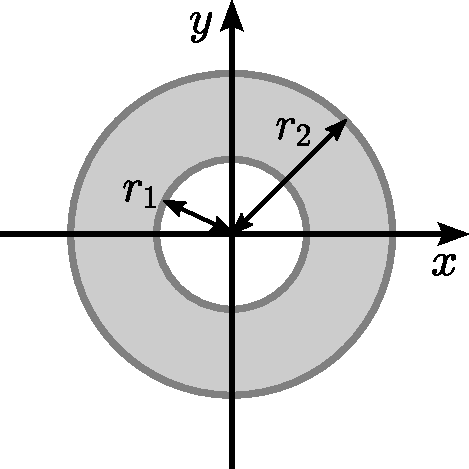
\includegraphics[scale=0.3]{moment_annulus}
\end{wrapfigure}
\begin{equation}
\begin{split}
EI(r) &= \underset{R}{\iint}E(r)y^2\,dA = \int_{r_1}^{r_2}\int_0^{2\pi} E(r)(r\sin\theta)^2(rdrd\theta)\\
&= \pi\int_{r_1}^{r_2} E(r)r^3 dr \qquad \text{Integrating over $\theta$}\\
\end{split}
\end{equation}
Therefore, specific flexural rigidity will be written as
\begin{equation}\label{objective_eb}
\begin{split}
strength(\chi) &=\frac{EI}{\rho}\\
&=\frac{\pi\sum^{r_o}_{r_i}E(r)r^3\Delta r}{2\pi r\sum^{r_o}_{r_i}\rho(r)\Delta r}\\
&=\frac{\sum^{r_o}_{r_i}E(r)r^3}{2 \sum^{r_o}_{r_i}\rho(r)r}
\end{split}
\end{equation}
where 
\begin{equation}
\begin{split}
E(r) &= \chi_1(r) E_1 + \chi_2(r) E_2\\
\rho(r) &= \chi_1(r) \rho_1 + \chi_2(r) \rho_2
\end{split}
\end{equation}
Here $\{E_1, \rho_1\}$ and $\{E_2, \rho_2\}$ are the material properties of the fibers and parenchyma respectively. $\chi_1$ and $\chi_2$ are the proportion of first and second material corresponding to fiber and parenchyma respectively.\par
Assuming small deformation, from Euler Bernoulli Beam Theory, we get strain $\varepsilon_{xx}$ as\\
Put Schematics for Beam Theory
\begin{equation}
\begin{split}
\varepsilon_{xx} &= \frac{\Delta x' - \Delta x}{\Delta x}\\
&= \frac{(R+y)\Delta\theta - R\Delta\theta}{R\Delta\theta}\\
&= \frac{y}{R}
\end{split}
\end{equation}
Therefore, using constitutive relation, we get $\sigma_{xx}$ as
\begin{equation}
\sigma_{xx} = E\varepsilon_{xx} = \frac{E}{R}y
\end{equation}
\begin{equation}\label{stress_eb}
\sigma = \frac{E}{R}r\sin\theta \quad (\because y = r\sin\theta)
\end{equation}
Now, moment can be written as
\begin{equation}\label{moment_eb}
\begin{split}
M(x) &= \int\int y\cdot\sigma(x,y)\cdot dydz\\
M &= \int_{r_i}^{r_o}\int_0^{2\pi}\sigma(r)r^2 sin\theta\,dr\,d\theta & \text{For a particular $x$}\\
&=\int_{r_i}^{r_o}\int_0^{2\pi} \frac{E(r)r sin\theta}{R}r^2 sin\theta\,dr\,d\theta &\quad (\text{From eqn }\eqref{stress_eb})\\
&=\pi\int_{r_i}^{r_o}\frac{r^3 E(r)}{R}\,dr
\end{split}
\end{equation}
\subsection{Optimization Problem}
Using \eqref{objective_eb}, \eqref{stress_eb}, \eqref{moment_eb}, the optimization problem becomes
\begin{equation}
\begin{split}
\underset{\chi}{max} \quad& \frac{\sum^{r_o}_{r_i}E(r)r^3}{\sum^{r_o}_{r_i}\rho(r)r}\\
s.t. \quad& \frac{rE(r)}{R}\leq \sigma_{max} \quad \forall r \in [r_i, r_o]\\
& \sum_{r_i}^{r_o}r^3E(r)\leq \frac{M_{max}R}{\pi\Delta r}
\end{split}
\end{equation}
\subsection{Cell Size}
For calculating parenchyma cell size, it is assumed that the cell thickness remains constant as we move from inner radius to the outer radius. The cell thickness has been determined from the dimensions given in Figure 4(a) in \cite{paper:mannan1}. \par
\begin{figure}[H]
\begin{center}
	\begin{tabular}{@{}c}
	\subfloat{
	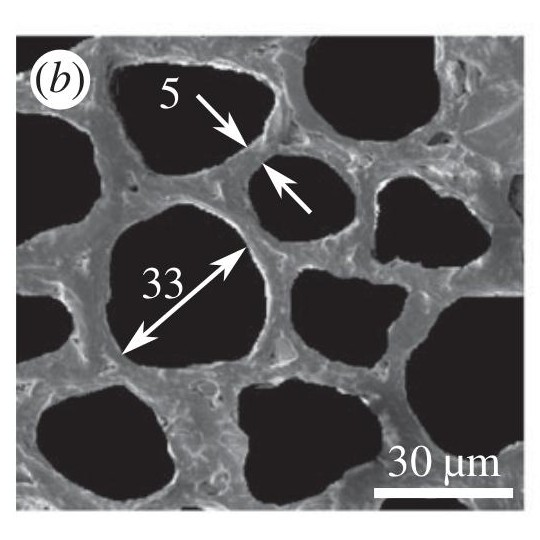
\includegraphics[scale=.3]{./Plots/cell/1.jpg}
	}
	\end{tabular}
%	\hfill
	\begin{tabular}{@{}c}
	\subfloat{
	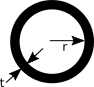
\includegraphics[scale=1.5]{./Plots/cell/scheme.png}
	}
	\end{tabular}
	
\caption{Cross-sectional micrograph showing the dimensions of typical parenchyma cell\label{fig:mannancell}
\cite{paper:mannan1}}
\end{center}
\end{figure}
Parenchyma cells consists of cellular material and air packets. Assuming cell to be spherical, let $v_a$ be the volume of air and $v_p$ be the volume of cellular material. From fig. \ref{fig:mannancell}

\begin{equation*}
v_a = \frac{4}{3}\pi r^3\\
v_p = \frac{4}{3}\pi 
\end{equation*}
\subsection{Results}
\subsubsection{Normal}
\begin{figure}[H]
\begin{center}
%     \subfloat[First sub-figure\label{subfig-1:radial}]{%
%		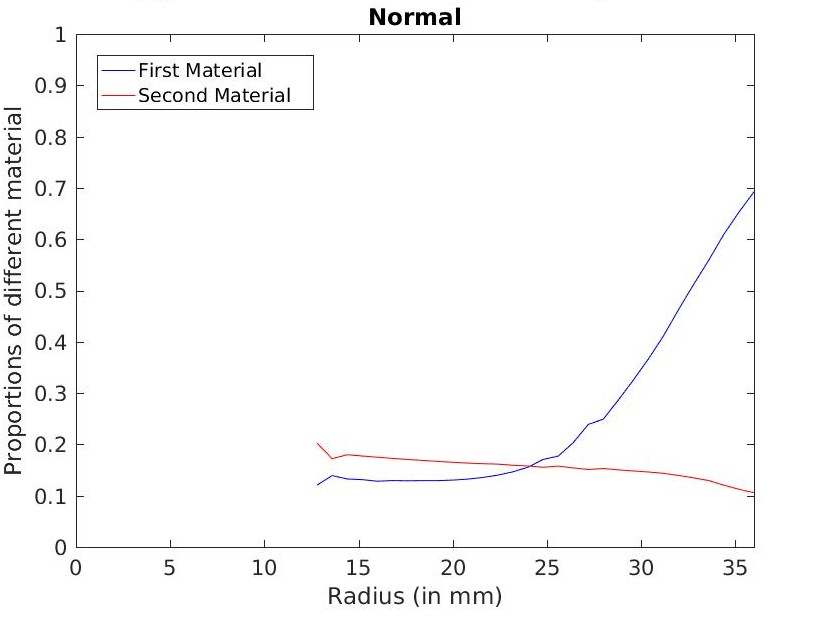
\includegraphics[scale=0.45]{./Plots/normal/a77_1.jpg}
%     }
%     \vfill
%     \subfloat[First sub-figure\label{subfig-2:radial}]{%
%       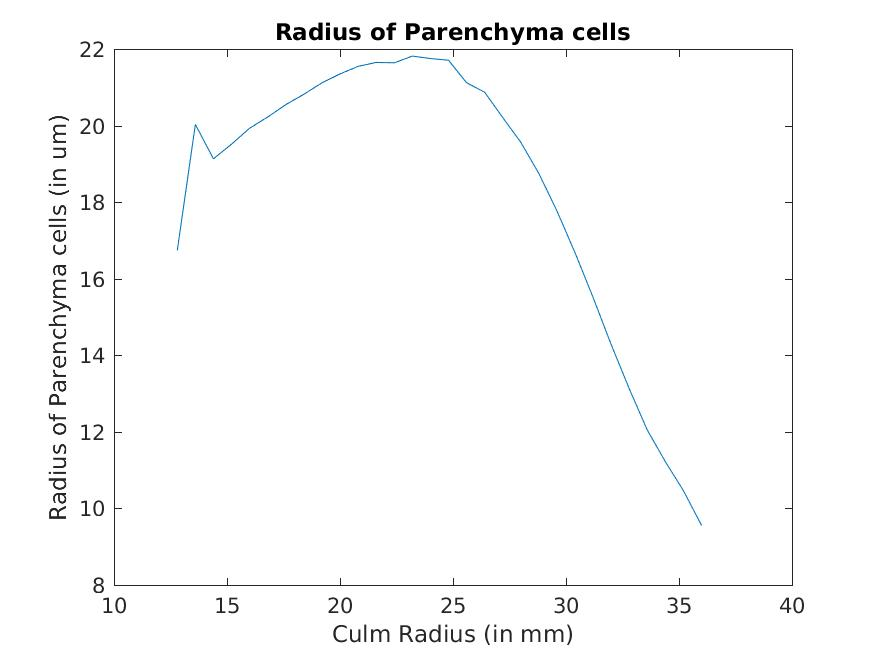
\includegraphics[scale=0.4]{./Plots/normal/b77.jpg}
%     }
	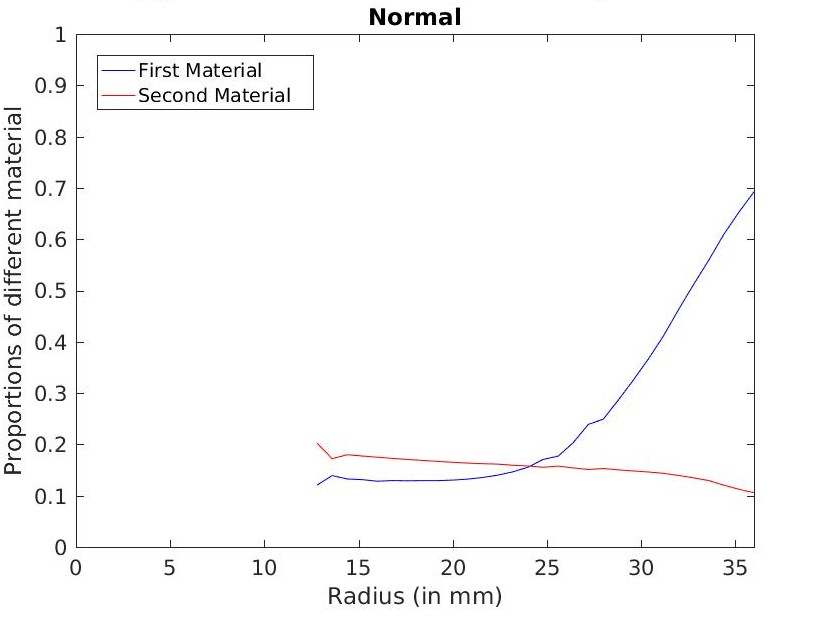
\includegraphics[scale=0.3]{./Plots/normal/a77_1.jpg}
	\label{fig:radial}
	\caption{Axisymmetric radial distribution of fibres and parenchyma obtained for an annular rod with inner radius 12mm and outer radius 36mm with $\sigma_{max} = $ 28MPa and $M_{max} = $ 580 N-m}
\end{center}
\end{figure}
\begin{figure}[H]
\begin{center}
	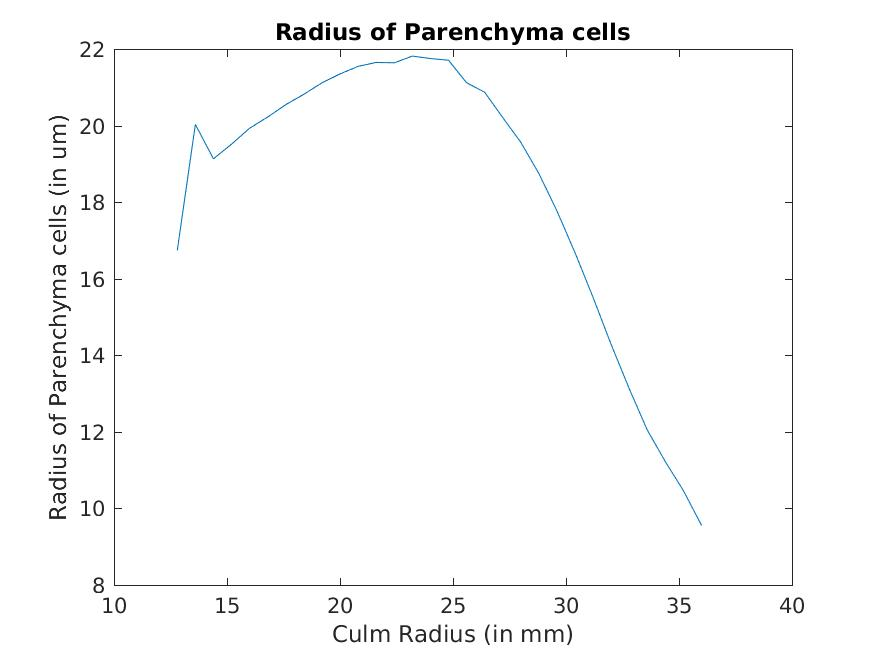
\includegraphics[scale=0.3]{./Plots/normal/b77.jpg}
	\label{fig:cellsize}
	\caption{Radius of parenchyma cell size obtained for an annular rod with inner radius 12mm and outer radius 36mm with $\sigma_{max} = $ 28MPa and $M_{max} = $ 580 N-m}
\end{center}
\end{figure}

\subsubsection{Extreme}
We have also obtained results for different types of bamboos, like bamboos with large cross-sectional diameter but thin annular cross-section and bamboos with small diameter but solid cross section with no hollow center.\par
It should be noted that we didn't have the experimental data for the set of constraint for these cases of bamboos. To obtain these constraints we first provide a rough estimate using the Euler Bernoulli beam equation. Then if the obtained variation of parenchyma cell size goes beyond what is generally observed in nature that set of constraints are rejected and the optimization problem is solved for a new set of sequentially generated constraints. This process is repeated untill a variation of cell size consistent with nature is observed. 

\begin{figure}[H]
\begin{center}
     \subfloat[\label{subfig-1:extreme1}]{%
		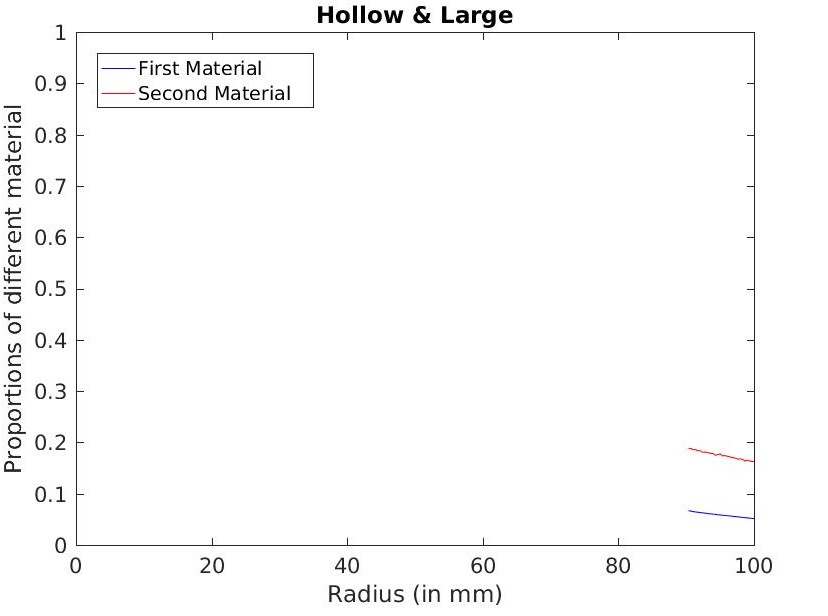
\includegraphics[scale=0.24]{./Plots/extremes/a53_1.jpg}
     }
     \hfill
     \subfloat[\label{subfig-2:extreme1}]{%
       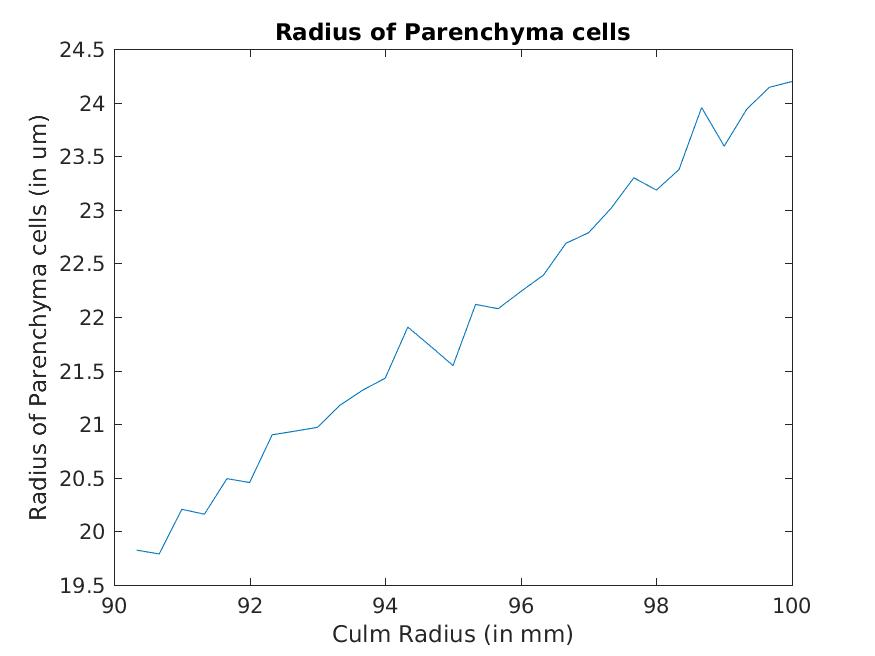
\includegraphics[scale=0.24]{./Plots/extremes/b53.jpg}
     }
	\label{fig:extreme1}
	\caption{(a)Axisymmetric radial distribution of fibres and parenchyma, (b)Radius of parenchyma cell size obtained for an annular rod with inner radius 90mm and outer radius 100mm with $\sigma_{max} = $ 150MPa and $M_{max} = $ 630 N-m}
\end{center}
\end{figure}

\begin{figure}[H]
\begin{center}
     \subfloat[\label{subfig-1:extreme2}]{%
		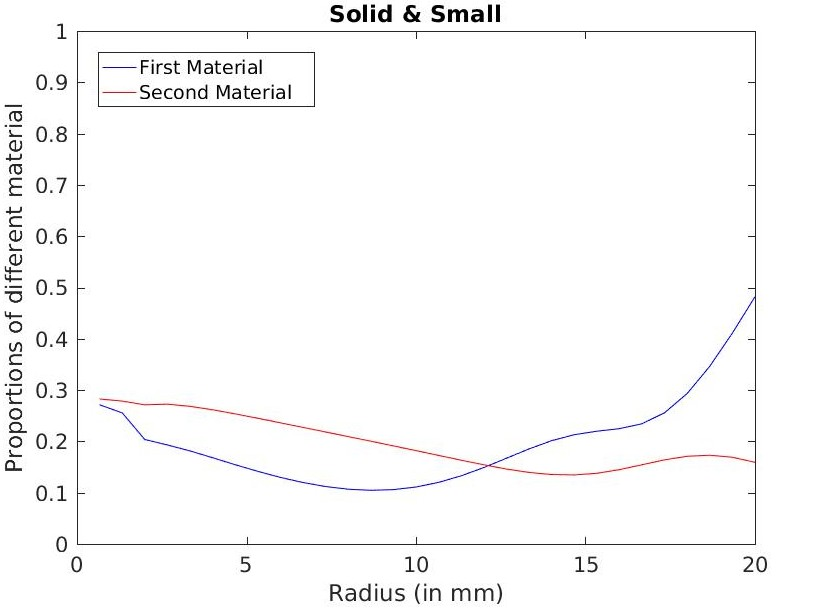
\includegraphics[scale=0.24]{./Plots/extremes/a63_1.jpg}
     }
     \hfill
     \subfloat[\label{subfig-2:extreme2}]{%
       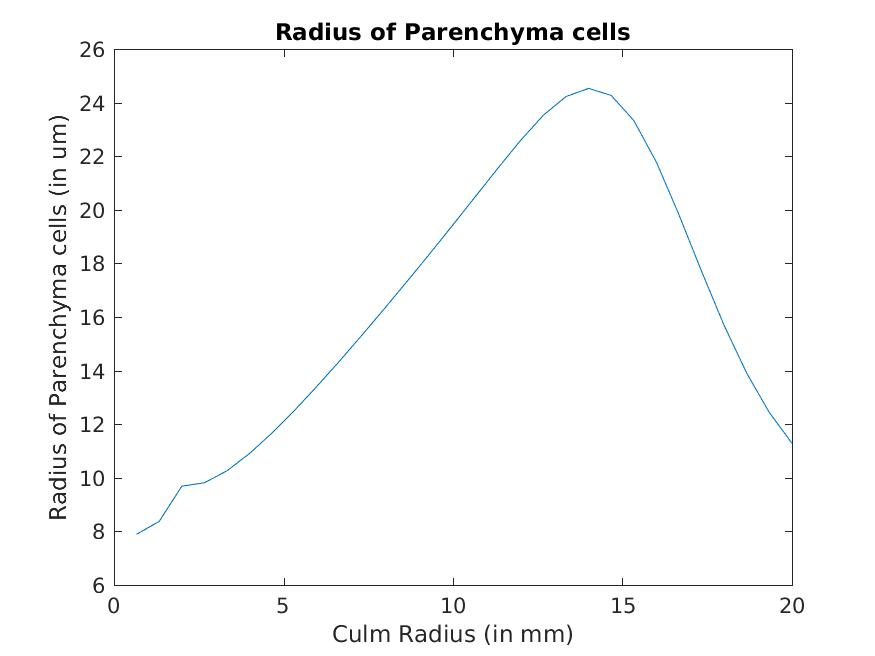
\includegraphics[scale=.24]{./Plots/extremes/b63.jpg}
     }
	\label{fig:extreme2}
	\caption{(a)Axisymmetric radial distribution of fibres and parenchyma, (b)Radius of parenchyma cell size obtained for an solid rod with radius 20mm with $\sigma_{max} = $ 24MPa and $M_{max} = $ 420 N-m}
\end{center}
\end{figure}
\subsubsection{Height}
\begin{figure}[H]
\begin{center}
	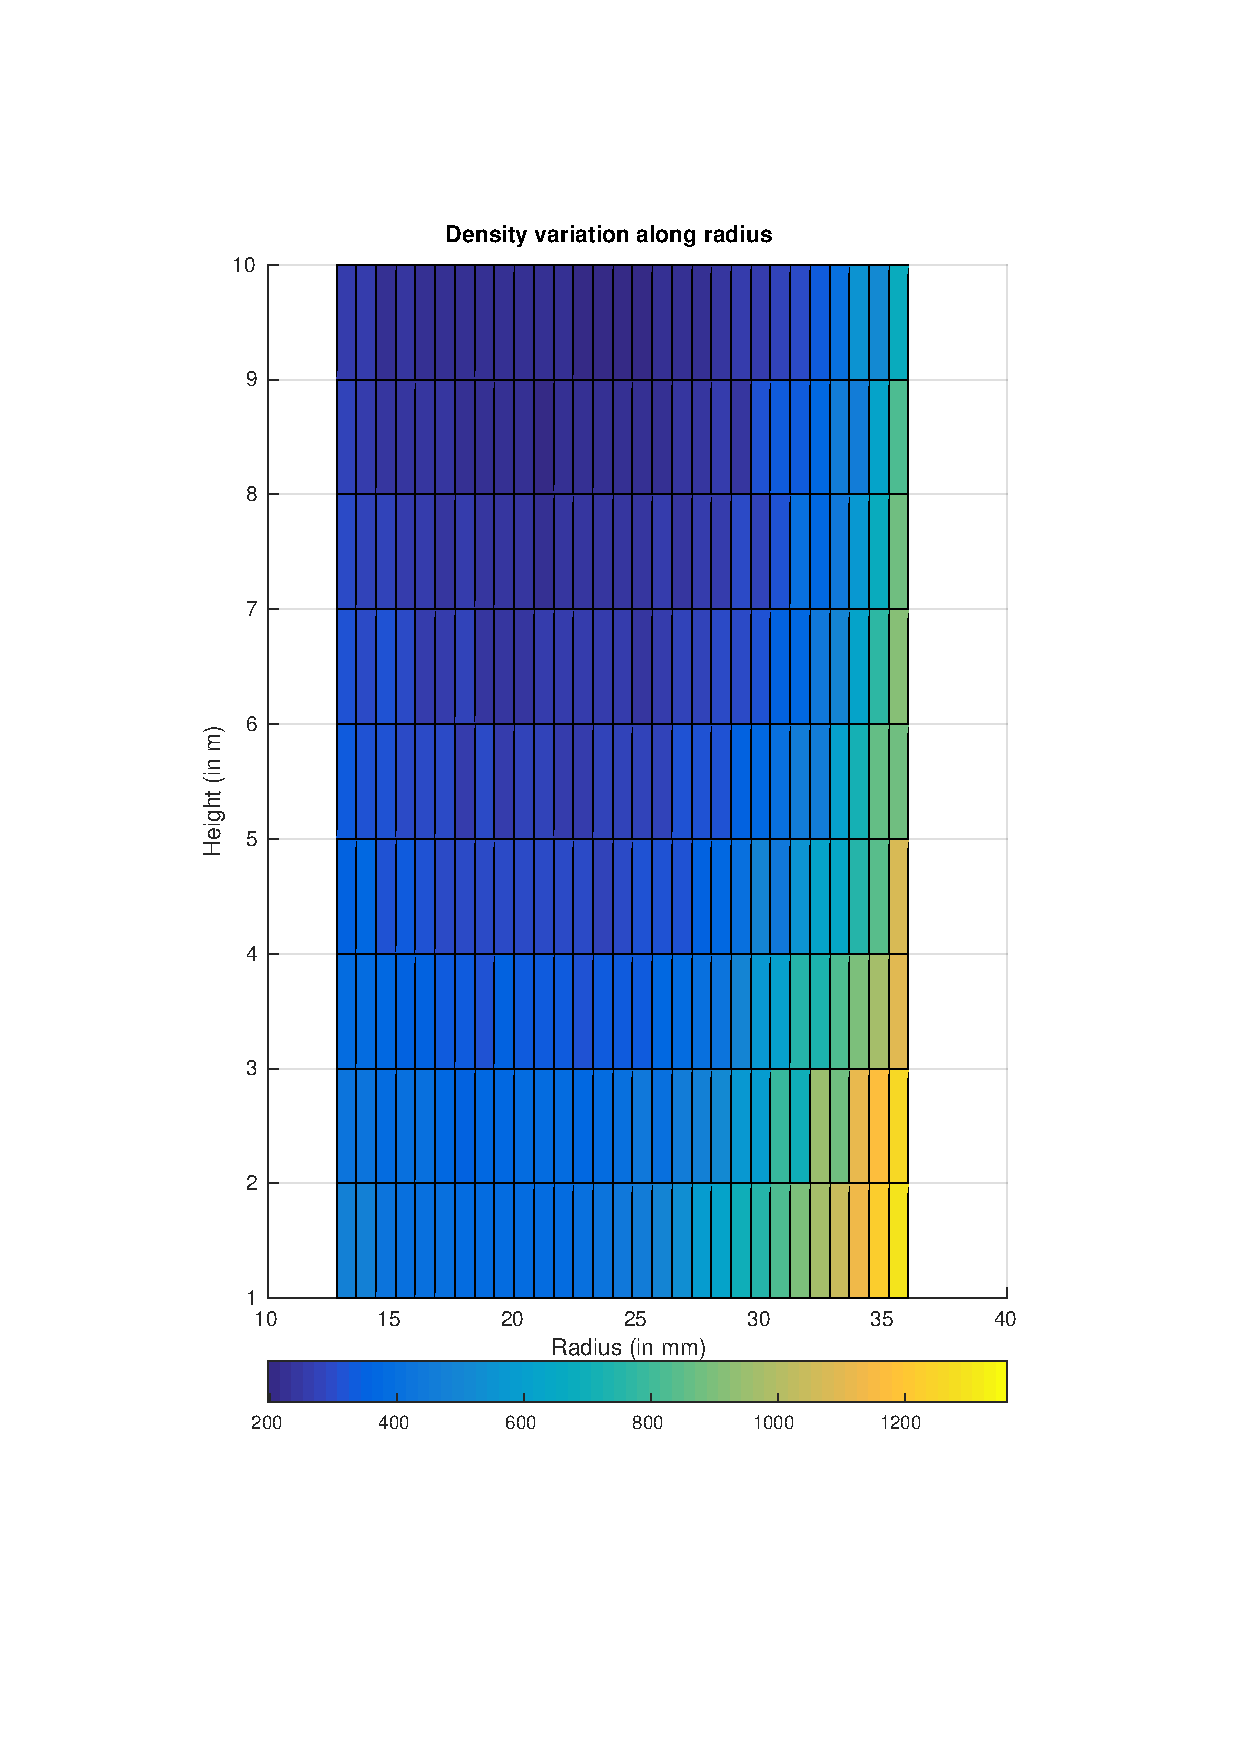
\includegraphics[clip, trim=2cm 5cm 2cm 3cm, scale=0.4]{./Plots/height/height.pdf}
	\label{fig:height}
	\caption{Density variation with height and radius obtained for an annular rod with inner radius 12mm and outer radius 36mm}
\end{center}
\end{figure}

\subsection{Conclusion}
Assuming axisymmetry, the radial distribution of constituent materials of bamboo is optimal for the constraints of maximum stress and bending moment that are applicable to bamboo under the loading conditions.

\newpage
\section{2D Simulation}
In the previous chapter, we discussed the optimality of the one-dimensional distribution of the given material of the bamboo for some constraints. To discuss the optimality of the structure originating from this one-dimensional distribution, we will first develop a process for generating optimal structures using topology optimization and finite element methods. Once, we have a sense of what an optimal structure for the given material and loading constraint, we can compare them with the structures found in natural bamboo and be able to comment on its optimality. So, in this chapter, we will discuss the topology optimization of the microstructure for the given constraints on macro-structure.
\par

\subsection{Overview}
First, an optimization problem is defined for minimizing the overall compliance of the structure with the constraints on volume. For calculating compliance ($\frac{1}{2}F^TU$), at every iteration, we find the displacement $U$ for given force $F$ and other boundary conditions on the macro domain. Displacements are determined by finite element analysis where the stiffness matrix for the macro domain elements is obtained by homogenization method. Each macro domain element is a called base cell and is further meshed to obtain the microstructure. To obtain the homogenized properties, another finite element analysis is done on this microdomain by applying periodic boundary conditions. It is the topology of this structure that we want to optimize. To achieve this, we link the optimality of the objective function to the topology of the microstructure through sensitivity analysis. For each element in the microdomain, a number is determined based on how critical is that element is for minimizing the objective function. After each iteration, the structure is updated based on the sensitivity numbers. This process is repeated until the volume constraint is achieved and the sensitivity numbers converge.

\subsection{Optimization Problem}
\begin{equation}
\label{eq:2dopt}
\begin{aligned}
& \underset{\chi}{\text{minimize :}}
& &  C = \frac{1}{2}\textbf{F}^\textbf{T}\textbf{U}\\
& \text{subject to:}
& & \sum_{j=1}^N V_j x_j - V_f = 0 \qquad \text{where }\quad x_j = \{0, 1\}
\end{aligned}
\end{equation}
Here, $\textbf{F}$ is the applied load, $\textbf{U}$ is the displacement of the macrostructure, $V_f$ is the specified volume fraction, $V_j$ is the volume of $j$th element of the base cell which has a total of $N$ elements. $x_j$ are the design variables represent the relative density. Element is made of material 1 for $x_j=1$ and material 2 for $x_j=0$. 

<Schematic of the cantilever beam>

<Schematic of the microstructure>

\subsection{Finite Element Analysis} 
The optimization problem defined in \eqref{eq:2dopt} requires the finite element analysis to be done on two scales, one for macrostructure and another for the base cell. For the microstructure, since the design variables can be either 0 or 1, Solid Isotropic Material with Penalization model\cite{paper:simp} is used for obtaining the material properties. Thus, the elasticity matrix can be written as
\begin{equation}
\label{eq:simp}
\textbf{D} = x_j^p\textbf{D}^1 + (1-x_j^p)\textbf{D}^2
\end{equation}
where $\textbf{D}^1$ and $\textbf{D}^2$ are the elasticity matrices for material 1 and 2 respectively, $p$ is the penalization constant.
For the macrodomain, we have the following FE equation
\begin{equation}
\textbf{KU} = \textbf{F}
\end{equation}
where $\textbf{K}$ is the assembled stiffness matrix for the macrostructure whose each component is calculated using
\begin{equation}
\label{eq:KM}
\textbf{K}_i =  \int_{V_i} \textbf{B}_i^T\textbf{D}_i^H\textbf{B}_i dV_i
\end{equation} 
where $\textbf{B}_i$ is the elemental strain-displacement matrix and $\textbf{D}_i^H$ is the homogenized elasticity matrix calculated from the finite analysis of the base cell. The homogenization process\cite{paper:homogenization} is discussed in the subsequent chapters. In this study, all base cells are assumed to be identical and therefore, equation \eqref{eq:KM} can be simplified as
\begin{equation}
\label{eq:KM1}
\textbf{K}_i =  \int_{V_i} \textbf{B}^T\textbf{D}^H\textbf{B} dV_i
\end{equation} 

\subsection{Periodic Boundary Conditions}
The process of homogenization requires the displacements corresponding to uniform strain fields, i.e., $[\epsilon_{11}, \epsilon_{22}, 2\epsilon_{12}] = [1, 0, 0]^T, [0, 1, 0]^T, [0, 0, 1]^T$. Periodic boundary conditions are needed to solve the finite element problem for uniform strain fields.\par
If $u$ and $v$ are the components of displacements in $p_1$ and $p_2$ directions respectively, then from periodicity, we have
%\begin{eqnarray}
%\label{eq:periodicity1}
%u(p_1, p_2) = u(p_1+P_1, p_2) = u(p_1, p_2+P_2) = u(p_1+P_1, p_2+P_2),\\
%\label{eq:periodicity2}
%v(p_1, p_2) = v(p_1+P_1, p_2) = v(p_1, p_2+P_2) = v(p_1+P_1, p_2+P_2).
%\end{eqnarray}
\begin{equation}
\label{eq:periodicity}
\begin{split}
u(p_1, p_2) = u(p_1+P_1, p_2) = u(p_1, p_2+P_2) = u(p_1+P_1, p_2+P_2),\\
v(p_1, p_2) = v(p_1+P_1, p_2) = v(p_1, p_2+P_2) = v(p_1+P_1, p_2+P_2).
\end{split}
\end{equation}
For cases $[1, 0, 0]^T$ and $[0, 1, 0]^T$, from symmetry of loading and geometry w.r.t. $q_1$, we have
\begin{eqnarray}
\label{eq:symmetryq1u}
u(p_1, p_2^0) = u(p_1, p_2^0+P_2),\\
\label{eq:symmetryq1}
v(p_1, p_2^0) = -v(p_1, p_2^0+P_2).
\end{eqnarray}
Similarly, using the symmetry about $q_2$, we have
\begin{eqnarray}
\label{eq:symmetryq2}
u(p_1^0, p_2) = -u(p_1^0+P_1, p_2),\\
\label{eq:symmetryq2v}
v(p_1^0, p_2) = v(p_1^0+P_1, p_2).
\end{eqnarray}
From eqs \eqref{eq:symmetryq1}, \eqref{eq:symmetryq2}, and \eqref{eq:periodicity}, we get
\begin{eqnarray}
\label{eq:fbc1}
u(p_1^0, p_2) = u(p_1^0+P_1, p_2) = 0,\\
\label{eq:fbc2}
v(p_1, p_2^0) = v(p_1, p_2^0+P_2) = 0.
\end{eqnarray}
Eqs \eqref{eq:symmetryq1u}, \eqref{eq:symmetryq2v}, \eqref{eq:fbc1} and 
\eqref{eq:fbc2} are the required periodic boundary conditions for strain fields $[1, 0, 0]^T$ and $[0, 1, 0]^T$.
\par
Now, For the case of $[0, 0, 1]^T$, loading is anti-symmetric and geometry is symmetric w.r.t. $q_1$ and $q_2$, as a result, we have
\begin{eqnarray}
\label{eq:symmetryq1u}
u(p_1, p_2^0) = -u(p_1, p_2^0+P_2),\\
\label{eq:symmetryq1}
v(p_1, p_2^0) = v(p_1, p_2^0+P_2).\\
\label{eq:symmetryq2}
u(p_1^0, p_2) = u(p_1^0+P_1, p_2),\\
\label{eq:symmetryq2v}
v(p_1^0, p_2) = -v(p_1^0+P_1, p_2).
\end{eqnarray}
From eqs \eqref{eq:symmetryq1u}, \eqref{eq:symmetryq2v}, and \eqref{eq:periodicity}, we get
\begin{eqnarray}
\label{eq:fbc2}
u(p_1, p_2^0) = u(p_1, p_2^0+P_2) = 0,\\
\label{eq:fbc1}
v(p_1^0, p_2) = v(p_1^0+P_1, p_2) = 0.
\end{eqnarray}
Eqs \eqref{eq:symmetryq1}, \eqref{eq:symmetryq2}, \eqref{eq:fbc1} and 
\eqref{eq:fbc2} are the required periodic boundary conditions for strain field $[0, 0, 1]^T$.\par
<Put schemtics of bc for first, second case>\\
<Put schemtics of bc for third case>\\
<Put deformation plots for each>\\

\subsubsection{Penalty Method}
We have used the penalty method to enforce the above discussed boundary conditions. Let these conditions on the displacements $\{\e U\}$ can be written as
\begin{equation*}
[\textbf{C}]\{\textbf{U}\} = \{\textbf{Q}\}
\end{equation*}
where $[\textbf{C}]$ and $\{\textbf{Q}\}$ are constants. Let us define $\{\textbf{t}\}$ as
\begin{equation*}
\{\textbf{t}\} = [\textbf{C}]\{\textbf{U}\} - \{\textbf{Q}\}
\end{equation*}
such that $\{\textbf{t}\} = \{\textbf{0}\}$ implies that the constraints are satisfied. Any non-negative values of $\{\textbf{t}\}$ must be penalized to minimize the violation of constraints. This is achieved by augmenting the potential energy function\cite{Book:Cook} $\Pi$ with a \textit{penalty function} $\frac{1}{2}\{\textbf{t}\}^T[\bm\alpha]\{\textbf{t}\}$, where $[\bm\alpha]$ is a diagonal matrix of penalty numbers. Thus, potential energy function becomes
\begin{equation}
\bm\Pi = \frac{1}{2}\{\e U\}^T[\e K]\{\e U\} - \{\e U\}^T\{\e F\} + \frac{1}{2}\{\textbf{t}\}^T[\bm\alpha]\{\textbf{t}\}
\end{equation}
where $[\e K]$ is the stiffness matrix and $\{\e F\}$ are the forces.\par
For minimum potential energy condition, $\{\frac{\partial\bm\Pi}{\partial\e U}\} = \{0\}$, this implies
\begin{equation}
\label{eq:penalty}
\bigg([\e K]+[\e C]^T[\bm\alpha][\e C]\bigg)\{\e U\} = \{\e F\} + [\e C]^T[\bm\alpha]\{\e Q\}
\end{equation}
If $[\bm\alpha]$ is null matrix, all constraints are ignored, else if $\alpha_i$'s are infinite, all constraints are satisfied. For a positive definite $[\e K]$, positive penalty numbers are used. We have set all penalty numbers to be same, this means that all constraints are given equal priority, i.e. $[\bm\alpha] = \alpha[I]$. $\alpha$ must be significantly larger to ensure that the constraint violation is negligible. Thus, the eq. \eqref{eq:penalty} reduces to the following
\begin{equation}
\label{eq:penalty1}
\bigg([\e K]+\alpha[\e C]^T[\e C]\bigg)\{\e U\} = \{\e F\} + \alpha[\e C]^T\{\e Q\}
\end{equation}
Eq \eqref{eq:penalty1} has to be solved separately for the three cases of periodic boundary conditions.

\subsection{Homogenization}
The homogenization method is generally used to analyze the properties of composites with complex but periodic microstructure. The procedure replaces the composites with an equivalent homogeneous material. 
The method is based on the two-scale asymptotic expansion of structural responses.

%The idea of asymptotic homogenization.
%In a repeating cell Y,
%\begin{equation}
%	\label{First}
%	\sigma_{ij} = C_{ijkl}\epsilon_{kl}	
%\end{equation}
%where $C_{ijkl}(\textbf{x}+\textbf{u}\textbf{Y})=C_{ijkl}(\textbf{x})$
%\begin{equation}
%\Rightarrow C_{ijkl}(x_1+n_1Y_1\, x_2+n_2Y_2\,x_3+n_3Y_3) = C_{ijkl}(x_1,x_2,x_3)
%\end{equation}
%$C_{ijkl}(\textbf{x}) $ is Y-periodic
%\begin{eqnarray}
%&\textbf{y} = \frac{\textbf{x}}{\epsilon}\\
%&\Rightarrow g = g(\textbf{x},\frac{\textbf{x}}{\epsilon}) = g(\textbf{x} \,\textbf{y})
%\end{eqnarray}
%$\textbf{x} = (x_1, x_2, x_3) \in \mathbb{R}^3$ defines the domain of the composite $\Omega$. The domain is composed of base cells of dimensions, $\varepsilon Y_1 , \varepsilon Y_2,\varepsilon Y_3$ where $\textbf{y}=\frac{\textbf{x}}{\varepsilon}$
%\subsubsection{1D Elasticity}
%\begin{eqnarray}
%&\sigma^\varepsilon = E^\varepsilon\frac{\partial u^\varepsilon}{\partial x}\\
%&\frac{\partial \sigma^\varepsilon}{\partial x}+\gamma^\varepsilon=0 & E^\varepsilon \, \gamma^\varepsilon \rightarrow macroscopically uniform
%\end{eqnarray}
%Inside each cell, 
%\begin{eqnarray}
%E^\varepsilon (x, \frac{x}{\varepsilon})&=E(y) \\ 
%\gamma^\varepsilon(x, \frac{x}{\varepsilon})&=\gamma(y)
%\end{eqnarray} 
%Let
%\begin{eqnarray}
%u^\varepsilon(x)=u^0{x,y}+\varepsilon u^1(x,y)+\varepsilon^2 u^2(x,y)+ ...\\
%\sigma^\varepsilon(x)=\sigma^0{x,y}+\varepsilon \sigma^1(x,y)+\varepsilon^2 \sigma^2(x,y)+ ...
%\end{eqnarray}


%\subsubsection{Optimal Design of Elastic structures}
%
%\begin{center}
%$\textbf{b} \rightarrow$ body forces\\
%$\textbf{t} \rightarrow$ surface tractions
%\end{center}
%
%Optimal choice of $\mathbb{C}_{ijkl} \in U_{ad} \leftarrow $ admissible set of elasticity \par $\mathbb{C}_{ijkl}(\textbf{x}) \forall \textbf{x} \in \Omega $ has 21 independent components \par $a_E(\textbf{u}, \textbf{v}) = \int_\Omega \mathbb{C}_{ijkl}\,\varepsilon_{kl}(\textbf{u})\,\varepsilon_{kl}(\textbf{v})d\textbf{v} \rightarrow $ energy bilinear form \par
%$L(\textbf{v}) = \int_\Omega \textbf{v}\, d\textbf{x}+\int_{\partial\Omega_t} \textbf{t}\cdot\textbf{v}ds \rightarrow $ load linear form.\par
%\hfill \break
%Minimum compliance problem:
%\begin{eqnarray}
%minimize & L(\textbf{v}),\\
%subject\, to & \mathbb{C}_{ijkl} \in \mathbb{U}_{ad}\\
%		  & a_E(\textbf{u}, \textbf{v}) = L(\textbf{v}) &\forall \textbf{v} \in \mathbb{U} 
%\end{eqnarray}
%where $\mathbb{U}\rightarrow $ kinematically admissible displacements.\\
%For optimal shape design:
%\begin{eqnarray}
%\mathbb{C}_{ijkl}(\textbf{x}) = \chi(\textbf{x})\overline{\mathbb{C}}_{ijkl}, & \textrm{where  } \overline{\mathbb{C}}_{ijkl}\rightarrow\textrm{stiffness matrix of the material}\\
%\chi(\textbf{x}) =
%    \begin{cases}
%        1 & \text{if $\textbf{x}\in \Omega^m$,}\\
%        0 & \text{if $\textbf{x}\in \Omega\backslash\Omega^m$}
%    \end{cases}
%\end{eqnarray}
%where $\Omega^m \rightarrow$ part of the domain occupied by the material.\\
%For sizing problem:
%\begin{eqnarray}
%\mathbb{C}_{ijkl}(\textbf{x}) = h(\textbf{x})\overline{\mathbb{C}}_{ijkl}\\
%& \int_\Omega \chi(\textbf{x})d\textbf{x}=V_f\\
%\& & \int_\Omega h(\textbf{x})d\textbf{x}=V_f.
%\end{eqnarray}
%where $h(x)$ is a sizing function. \hfill
%\break
%Traditionally shape design problems are initiated in the following manner:
%\begin{align}
%Ref\, doamin: & \Omega_0\in \mathbb{R}^3\\
%\underline{\phi}:  & \Omega_0 \rightarrow \phi(\Omega_0) \text{is a diffeomorphism.}\\
%L(\textbf{v})&=\int_{\Omega_0} \textbf{f}\cdot\textbf{v} |det(D\underline{\phi}^{-1})|d\textbf{x}+\int_{\partial\Omega_t} \textbf{t}\cdot\textbf{v}|det(D\underline{\phi}^{-1})|ds
%\end{align}
%
%\begin{equation}
%\begin{split}
%a_E &=\int_\Omega \mathbb{C}_{ijkl}(\textbf{x}\varepsilon_{kl}(\textbf{v})\varepsilon_{ij}(\textbf{v})d\textbf{x}\\
%&=\int_{\Omega_0} \mathbb{C}_{ijkl}\varepsilon_{kl}(\textbf{v})\varepsilon_{ij}(\textbf{v})|det(D\underline{\phi}^{-1})|d\textbf{x}
%\end{split}
%\end{equation}
%
%Now,
%\begin{equation}	\label{compliance}
%\begin{split}
%\mathbb{C}_{ijkl} \varepsilon_{kl} &= \mathbb{C}_{ijkl}\frac{1}{2}(u_{k,l}+u_{l,k})\\
% & =\frac{1}{2}\mathbb{C}_{ijkl}u_{k,l}+\frac{1}{2}\mathbb{C}_{ijlk}u_{l,k}\\
% & =\mathbb{C}_{ijkl}u_{k,l}
%\end{split}
%\end{equation}
%\begin{equation}
%\begin{split}
%a_E &= \int_{\Omega_0}\mathbb{C}_{ijkl}u_{k,l}(\textbf{u})u_{i,j}(\textbf{v})|det(D\underline{\phi}^{-1}|d\textbf{x}\\
%&= \int_{\Omega_0}\mathbb{C}_{ijkl}\frac{\partial u_k}{\partial\textbf{x}_m}(D\underline{\phi}^{-1})_{ml}\frac{\partial u_i}{\partial \textbf{x}_p}(D\phi^{-1})_{pj}|det(D\underline{\phi}^{-1})|d\textbf{x}\\
%\end{split}
%\end{equation}
%\begin{eqnarray}
%\Rightarrow \mathbb{C}_{ijkl}(D\underline{\phi}^{-1})_{ml}(D\underline{\phi}^{-1})_{pj}|det(D\underline{\phi}^{-1})| = \bar{\mathbb{C}}_{ipkm}\\
%\bar{\mathbb{C}}_{ijkl} = \mathbb{C}_{ipkm}(D\underline{\phi}^{-1})_{lm}(D\underline{\phi}^{-1})_{jp}|det(D\underline{\phi}^{-1})|
%\end{eqnarray}
%Treating $\underline{\phi}$ as a design variable is tedious.
%
We will now derive the equation for homogenization. 
%From Cauchy's First law of motion
%\begin{equation}
%\label{eq:cauchy}
%\frac{\partial \sigma_{ij}}{\partial x_i} + f_j = 0
%\end{equation}
%where $\sigma_{ij} = E_{ijkl}\epsilon_{kl}$ and $\e f$ are the forces. Now $\epsilon_{kl} = \frac{1}{2}(\fj{u_k}{x_l}+\fj{u_l}{x_k})$. Also, in the SIMP material model, $E_{ijkl}$ is function of $\e x$.
%So, eq \eqref{eq:cauchy} can be written as
%\begin{eqnarray}
%\label{eq:cauchy1}
%\fj{}{x_i}\bigg(E_{ijkl}(\e x)(\fj{u_k}{x_l}+\fj{u_l}{x_k})\bigg) + f_j &= 0 \qquad &\text{in } \Omega
%%\e u^\varepsilon \big|_{\partial\Omega} &= 0 \qquad &\text{on } \partial \Omega
%\end{eqnarray}
Now, the structure is Y-periodic, therefore we have, $E_{ijkl}(\e y) =E_{jikl}(\e y) =E_{ijlk}(\e y) =E_{klij}(\e y)$ where $\e y = \e x/\varepsilon$
\begin{figure}[H]
\begin{center}
	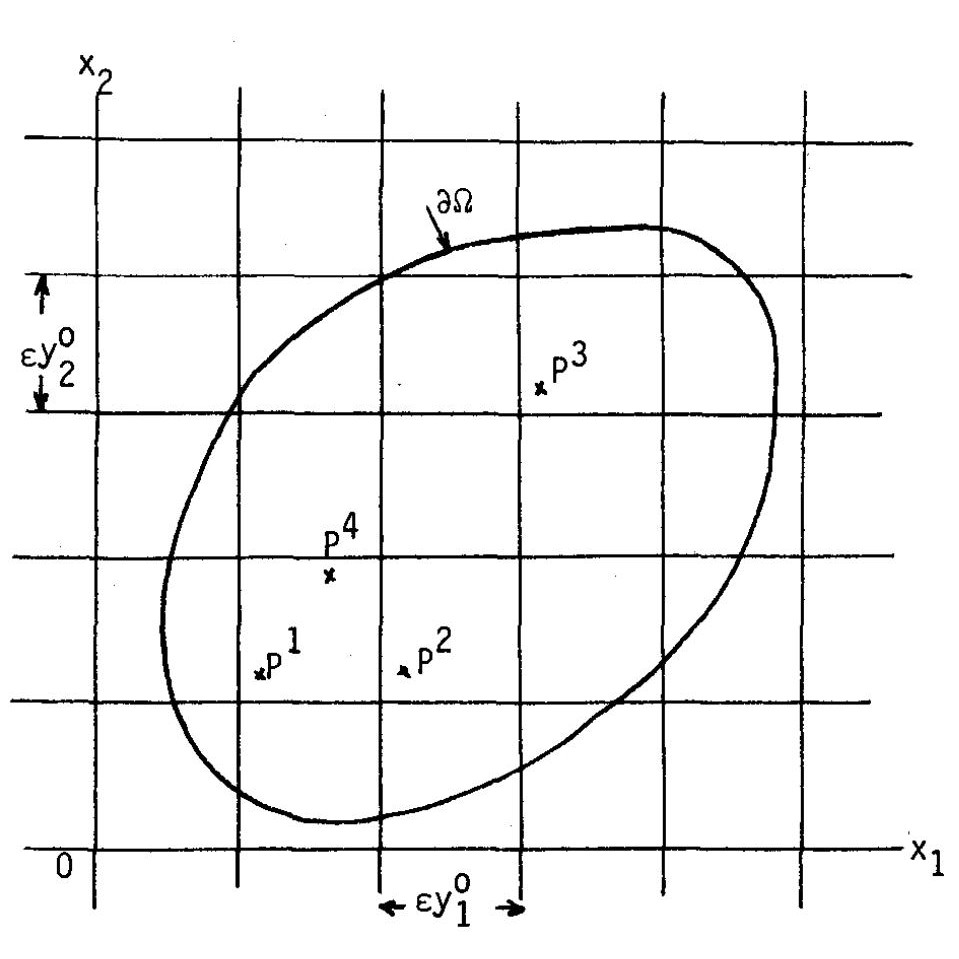
\includegraphics[scale=0.2]{./Plots/homo/2.jpg}
	\label{fig:doublescale}
	\caption{Schematic for periodic structure and double scale modeling}
\end{center}
\end{figure}
$E_{ijkl}(\e y)$ is assumed to satisfy strong ellipticity condition, i.e., there exists $m>0$ such that.
\begin{gather}
\sum_{i,j,k,l=1}^N E_{ijkl}^\varepsilon(x)\textbf{X}_{ij}\textbf{X}_{kl}\geq m\sum_{i,j=1}^N\textbf{X}_{ij}\textbf{X}_{ij} \qquad \forall \quad \textbf{X}_{ij}=\textbf{X}_{ji}
\end{gather}
Let us define
\begin{equation}
E_{ijkl}^\varepsilon (\textbf{x}) = E_{ijkl}(\textbf{x},\textbf{y}), \qquad \textbf{y} = \frac{\textbf{x}}{\varepsilon}
\end{equation}
%Therefore, eq \eqref{eq:cauchy1} becomes
%\begin{equation}
%\label{eq:cauchy1}
%\fj{}{x_i}\bigg(E_{ijkl}^\varepsilon(\e x)(\fj{u_k^\varepsilon}{x_l}+\fj{u_l^\varepsilon}{x_k})\bigg) + f_j = 0
%\end{equation}
%Now, let us suppose there exist $\e u$ and $\e v$ which satisfy the periodic boundary conditions\par
Let the domain $\Omega$ has a boundary $\Gamma$. Let $\textbf{f}$ be the body force acting on $\Omega$ and $\textbf{t}$ be the traction acting on $\Gamma_t$ part of the boundary $\Gamma$. Also, let $\Gamma_D$ be the part of boundary on which displacement is defined. Then the displacement $\textbf{u}^\varepsilon$ can be obtained as the solution to the following minimization problem
\begin{align}
\label{fem}
\min_{\textbf{v}^\varepsilon\in U} \quad F^\varepsilon(\textbf{v}^\varepsilon),
\end{align} 
where $F^\varepsilon$ is total potential energy given as	
\begin{eqnarray} \label{tpe}
F^\varepsilon(\textbf{v}^\varepsilon) = \frac{1}{2}\int_\Omega E^\varepsilon_{ijkl}(\e x)\epsilon_{kl}(\textbf{v}^\varepsilon)\epsilon_{ij}(\textbf{v}^\varepsilon)dx-\int_\Omega\textbf{f}\cdot\textbf{v}^\varepsilon dx - \int_{\Gamma_t}\textbf{t}\cdot\textbf{v}^\varepsilon ds
%F^\varepsilon(\textbf{v}^\varepsilon) = \frac{1}{2}a^\varepsilon(\textbf{v}^\varepsilon, \textbf{v}^\varepsilon)-L(\textbf{v}^\varepsilon),\\
%a^\varepsilon(\textbf{u},\textbf{v})=\int_\Omega E^\varepsilon_{ijkl}\varepsilon_{kl}(\textbf{u})\varepsilon_{ij}(\textbf{v})dx,\\
%L(\textbf{v})=\int_\Omega\textbf{f}\cdot\textbf{v}dx + \int_{\Gamma_t}\textbf{t}\cdot\textbf{v}ds
\end{eqnarray}
and $\mathcal{U}$ is the set of admissible displacements defined such that
\begin{equation}
\mathcal{U} = \{\textbf{v} = v_i\textbf{e}_i :\, v_i\in H^1(\Omega) \text{ and } \textbf{v}\in\mathcal{G} \text{ on } \Gamma_D\}
\end{equation}
where $\mathcal{G}$ is set of displacement defined along the boundary $\Gamma_D$.\\
Let 
\begin{align}
\textbf{v}^\varepsilon(\textbf{x}) = \textbf{v}^0(\textbf{x})+\varepsilon\textbf{v}^1(\textbf{x},\textbf{y}),\qquad \textbf{y}=\frac{\textbf{x}}{\varepsilon}.
\end{align}
Using chain rule for functions in two variables\\
\begin{equation}
\begin{split}
\frac{\partial f(\e x, \e y(\e x))}{\partial \textbf{x}} &= \frac{\partial f}{\partial \textbf{x}}+\frac{\partial f}{\partial \textbf{y}}\frac{\partial \textbf{y}}{\partial \textbf{x}}\\
&=\frac{\partial f}{\partial \textbf{x}}+\frac{1}{\varepsilon}\frac{\partial f}{\partial \textbf{y}}
\end{split}
\end{equation}
Using above two equations, we can write the linerized strain as
\begin{equation}
\begin{split}
\epsilon_{ij}(\textbf{v}^\varepsilon(\textbf{x})) &= \frac{\partial (v_{i}^0(\textbf{x})+\varepsilon v_{i}^1(\textbf{x},\textbf{y}))}{\partial x_j}\\
&=\frac{\partial v_i^0}{\partial x_j}+\varepsilon\bigg\{\frac{\partial v_{i}^1}{\partial x_j}+\frac{1}{\varepsilon}\frac{\partial v_{i}^1}{\partial y_j}\bigg\}\\
&\approx \frac{\partial v_{i}^0}{\partial x_j}+\frac{\partial v_{i}^1}{\partial y_j} &\qquad \{ \varepsilon << 1\}
\end{split}
\end{equation}
Therefore, equation \eqref{tpe} can be written as 
\begin{multline}
F^\varepsilon(\textbf{v}^\varepsilon) = \frac{1}{2}\int_\Omega E^\varepsilon_{ijkl}(\e x)\bigg (\frac{\partial v_{k}^0}{\partial x_l}+\frac{\partial v_{k}^1}{\partial y_l}\bigg )\bigg (\frac{\partial v_{i}^0}{\partial x_j}+\frac{\partial v_{i}^1}{\partial y_j}\bigg )dx\\
-\int_\Omega\textbf{f}\cdot\textbf{v}^0 dx - \int_{\Gamma_t}\textbf{t}\cdot\textbf{v}^0 ds + \varepsilon R^\varepsilon(\textbf{v}^0, \textbf{v}^1)
\end{multline}
Here, $R^\varepsilon$ is the contribution of $\varepsilon\textbf{v}^1$ in the calculation of energy from body force and traction.
Using average operator 
\begin{equation}
\Phi^\varepsilon(\e x) = \frac{1}{|Y|}\int_Y \Phi(\e x,\e y)dy,
\end{equation}
%\begin{equation}
%\lim_{\varepsilon\rightarrow 0}\int_\Omega \Phi(x, x/\varepsilon)dx = \frac{1}{|Y|}\int_\Omega\int_Y \Phi(x,y)dydx,
%\end{equation}
we get,
\begin{equation}
\begin{split}
%\lim_{\varepsilon\rightarrow 0}
\,F^\varepsilon(\textbf{v}^\varepsilon)&=F(\textbf{v}^0,\textbf{v}^1)\\
&=\frac{1}{2|Y|}\int_\Omega\int_Y E_{ijkl}(\e x,\e y) \bigg (\frac{\partial v_{k}^0}{\partial x_l}+\frac{\partial v_{k}^1}{\partial y_l}\bigg )\bigg (\frac{\partial v_{i}^0}{\partial x_j}+\frac{\partial v_{i}^1}{\partial y_j}\bigg )dy\,dx\\
&\qquad-\int_\Omega\textbf{f}\cdot\textbf{v}^0 dx - \int_{\Gamma_t}\textbf{t}\cdot\textbf{v}^0 ds 
\end{split}
\end{equation}
Let $\e u^\varepsilon\{\textbf{u}^0, \textbf{u}_1\}$ be a minimizer of the functional $F$, then 
\begin{eqnarray}
\label{eq:functional1}
%\begin{aligned}
\frac{1}{|Y|}\int_\Omega\int_Y E_{ijkl}(x,y)\bigg (\frac{\partial u_{k}^0}{\partial x_l}+\frac{\partial u_{k}^1}{\partial y_l}\bigg )\bigg (\frac{\partial v_{i}^0}{\partial x_j}\bigg ) dy\,dx = \int_\Omega\textbf{f}\cdot\textbf{v}^0 dx + \int_{\Gamma_t}\textbf{t}\cdot\textbf{v}^0 ds &\forall \textbf{v}^0\\
\label{eq:functional2}
\frac{1}{|Y|}\int_\Omega\int_Y E_{ijkl}(x,y)\bigg (\frac{\partial u_{k}^0}{\partial x_l}+\frac{\partial u_{k}^1}{\partial y_l}\bigg )\bigg (\frac{\partial v_{i}^1}{\partial x_j}\bigg ) dy\,dx = 0,  &\forall \textbf{v}^1
%\end{aligned}
\end{eqnarray}
Let $u_{k}^1$ be a function of directional derivative of $u^0$ times the displacement of the base cell element in that direction. Here $\chi$ is the microscopic displacement field which satisfies the condition of Y-periodicity.
\begin{equation}\label{localization}
u_{k}^1(x,y)=-\chi^{pq}_k(y)\frac{\partial u_{p}^0}{\partial x_q}(x),
\end{equation}
Then, eq \eqref{eq:functional2} becomes
\begin{align}
%&\int_\Omega\int_Y E_{ijkl}(x,y)\bigg (\frac{\partial u_{k}^0}{\partial x_l}-\frac{\partial \chi^{pq}_k}{\partial y_l}\frac{\partial u_{p}^0}{\partial x_q}\bigg )\frac{\partial v^1_{i}}{\partial x_j} dy\,dx=0\\
%&\int_\Omega\int_Y \bigg (E_{ijkl}\frac{\partial u_{0k}}{\partial x_l}-E_{ijkl}\frac{\partial \chi^{pq}_k}{\partial y_l}\frac{\partial u_{p}^0}{\partial x_q}\bigg )\frac{\partial v_{i}^1}{\partial x_j} dy\,dx=0\\
%&\int_\Omega\int_Y \bigg (E_{ijkl}\frac{\partial u_{0k}}{\partial x_l}-E_{ijpq}\frac{\partial \chi^{kl}_p}{\partial y_q}\frac{\partial u_{k}^0}{\partial x_l}\bigg )\frac{\partial v_{i}^1}{\partial x_j} dy\,dx=0\\
%&\int_\Omega\int_Y \frac{\partial u_{k}^0}{\partial x_l}\bigg (E_{ijkl}-E_{ijpq}\frac{\partial \chi^{kl}_p}{\partial y_q}\bigg )\frac{\partial v_{i}^1}{\partial x_j} dy\,dx=0\\
&\int_\Omega\frac{\partial u_{k}^0}{\partial x_l}dx\cdot\int_Y \bigg (E_{ijkl}-E_{ijpq}\frac{\partial \chi^{kl}_p}{\partial y_q}\bigg )\frac{\partial v_{i}^1}{\partial x_j} dy\,=0\\
\label{eq:homogenized1}
&\Rightarrow \int_Y \bigg (E_{ijkl}-E_{ijpq}\frac{\partial \chi^{kl}_p}{\partial y_q}\bigg )\frac{\partial v_{i}^1}{\partial x_j} dy=0  \qquad \text{for k, l = 1 and 2,}
\end{align}
%if $x^{pq}$ satifies
%\begin{equation}
%\int_Y \bigg ( E_{ijkl}-E_{ijpq}\frac{\partial \chi^{kl}_p}{\partial y_q}\bigg ) \frac{\partial v_{1j}}{\partial y_i}\,dy=0 \qquad \text{for k, l = 1 and 2,} 
%\end{equation}
Similarly, substituting equation \eqref{localization} in \eqref{eq:functional1} gives the homogenized equation.
\begin{align*}
\text{LHS}&=\frac{1}{|Y|}\int_\Omega\int_Y E_{ijkl}(x,y)\bigg (\frac{\partial u_{k}^0}{\partial x_l}+\frac{\partial u_{k}^1}{\partial y_l}\bigg )\bigg (\frac{\partial v_{i}^0}{\partial x_j}\bigg ) dy\,dx\\
&=\frac{1}{|Y|}\int_\Omega\int_Y \bigg (E_{ijkl}\frac{\partial u_{k}^0}{\partial x_l}-E_{ijpq}\frac{\partial \chi^{kl}_p}{\partial y_q}\frac{\partial u_{k}^0}{\partial x_l}\bigg )\frac{\partial v_{i}^0}{\partial x_j} dy\,dx\\
&=\frac{1}{|Y|}\int_\Omega\Bigg \{\int_Y \bigg (E_{ijkl}-E_{ijpq}\frac{\partial \chi^{kl}_p}{\partial y_q}\bigg )dy\Bigg \}\frac{\partial u_{k}^0}{\partial x_l}\frac{\partial v_{i}^0}{\partial x_j}dx\\
&=\int_\Omega E^H_{ijkl}(x)\frac{\partial u_{k}^0}{\partial x_l}\frac{\partial v_{i}^0}{\partial x_j}\,dx
\end{align*}
Homogenized equation
\begin{equation}
\int_\Omega E^H_{ijkl}(x)\frac{\partial u_{k}^0}{\partial x_l}\frac{\partial v_{i}^0}{\partial x_j}\,dx = \int_\Omega\textbf{f}\cdot\textbf{v}^0 dx + \int_{\Gamma_t}\textbf{t}\cdot\textbf{v}^0 ds \qquad \text{for every } \textbf{v}^0
\end{equation}
where $E^H_{ijkl}(x)$ is
\begin{equation}
\label{eq:homogenized}
\boxed{E^H_{ijkl} = \frac{1}{|Y|}\int_Y \bigg (E_{ijkl}-E_{ijpq}\frac{\partial \chi^{kl}_p}{\partial y_q}\bigg ) dy}
\end{equation}
%Now, Define
%\begin{eqnarray}
%a_H(\textbf{u},\textbf{v}) = \int_\Omega E^H_{ijkl}(\textbf{x})\frac{\partial u_k}{\partial x_l}\frac{\partial v_i}{\partial	x_j}\, dx,\\
%a_Y(\chi^{kl}, \textbf{v})=\int_Y E_{ijpq}(\textbf{x},\textbf{y})\frac{\partial \chi^{kl}_p}{\partial y_q}\frac{\partial v_i}{\partial y_j}\,dy,\\
%L^{kl}_Y(\textbf{v})=\int_Y E_{ijkl} \frac{\partial v_i}{\partial y_j}\, dy
%\end{eqnarray}
%At microscopic level, we have
%\begin{equation}\label{microscopic}
%a_Y(\chi^{kl}, \textbf{v}) = L_Y^{kl}(\textbf{v})\qquad \forall \textbf{v}\in \mathcal{U}_Y,
%\end{equation}
%At macroscopic level, we have
%\begin{equation}
%a_H(\textbf{u},\textbf{v}) = L(\textbf{v})\qquad \forall \textbf{v}\in \mathcal{U}_0
%\end{equation}
%where $\mathcal{U}_0$ is homogeneous case of $\mathcal{U}$, i.e., $\textbf{g}=0$.
\subsubsection{Implementation}
% 2D Homogenization}
%Basic homogenization equation, 
%\begin{equation}
%u_{i}^1(\textbf{x},\textbf{y}) = -\chi^{pq}_i\frac{\partial u_{p}^0(\textbf{x})}{\partial x_q}
%\end{equation}
%Solve $\chi^{kl}_p$ from:
%\begin{equation}
%\int_Y \bigg ( E_{ijkl} - E_{ijpq}\frac{\partial\chi^{kl}_p}{\partial y_q}\bigg ) \frac{\partial v_{i}^1}{\partial y_j}\,dy = 0
%\end{equation}
%Compute:
%\begin{equation}\label{homoE}
%E_{ijkl}^H=\frac{1}{|Y|}\int_Y\bigg (E_{ijkl} - E_{ijpq}\frac{\partial\chi^{kl}_p}{\partial y_q}\bigg )\,dy
%\end{equation}
%\subsubsection{Examples}
For 2D problems, it is sufficient to solve \eqref{eq:homogenized} for $i, j, p, q = \{1, 2\}$ and three cases for $\{k, l\} = \{1,1\}, \{2,2\}, \{1,2\}$. In this section, we will refer $\e v^1$ as $\e v$. Assuming orthotropicity, we solve eq \eqref{eq:homogenized1} for $\{k,l\} = \{1,1\}$ we get
%\begin{equation}\label{2drhs}
%\begin{split}
%\int_Y E_{ijkl}\frac{\partial v_i}{\partial y_j}\, dy &=\int_Y E_{ij11}\frac{\partial v_i}{\partial y_j}\,dy\\
%&=\int_Y\bigg (E_{1111}\frac{\partial v_1}{\partial y_1}+E_{2211}\frac{\partial v_2}{\partial y_2}\bigg )\, dy
%\end{split}
%\end{equation}
%\begin{equation}\label{2dlhs}
%\begin{split}
%\int_Y E_{ijpq}\frac{\partial \chi^{kl}_p}{\partial y_q}\frac{\partial v_i}{\partial y_j}\,dy &=\int_Y E_{ijpq}\frac{\partial \chi^{11}_p}{\partial y_q}\frac{\partial v_i}{\partial y_j}\,dy\\
%&=\int_Y \bigg \{ E_{11pq}\frac{\partial \chi^{11}_p}{\partial y_q}\frac{\partial v_1}{\partial y_1} + E_{12pq}\frac{\partial \chi^{11}_p}{\partial y_q}\frac{\partial v_1}{\partial y_2}\\
%&\qquad\qquad + E_{21pq}\frac{\partial \chi^{11}_p}{\partial y_q}\frac{\partial v_2}{\partial y_1} + E_{22pq}\frac{\partial \chi^{11}_p}{\partial y_q}\frac{\partial v_2}{\partial y_2}\bigg \}\,dy\\
%&=\int_Y \bigg \{\bigg ( E_{1111}\frac{\partial \chi^{11}_1}{\partial y_1} + E_{1112}\frac{\partial \chi^{11}_1}{\partial y_2} + E_{1121}\frac{\partial \chi^{11}_2}{\partial y_1} + E_{1122}\frac{\partial \chi^{11}_2}{\partial y_2}\bigg )\frac{\partial v_1}{\partial y_1}\\
%&\qquad + \bigg (E_{1211}\frac{\partial \chi^{11}_1}{\partial y_1} + E_{1212}\frac{\partial \chi^{11}_1}{\partial y_2} + E_{1221}\frac{\partial \chi^{11}_2}{\partial y_1} + E_{1222}\frac{\partial \chi^{11}_2}{\partial y_2}\bigg )\frac{\partial v_1}{\partial y_2}\\
%&\qquad + \bigg (E_{2111}\frac{\partial \chi^{11}_1}{\partial y_1} + E_{2112}\frac{\partial \chi^{11}_1}{\partial y_2} + E_{2121}\frac{\partial \chi^{11}_2}{\partial y_1} + E_{2122}\frac{\partial \chi^{11}_2}{\partial y_2}\bigg )\frac{\partial v_2}{\partial y_1}\\
%&\qquad + \bigg (E_{2211}\frac{\partial \chi^{11}_1}{\partial y_1} + E_{2212}\frac{\partial \chi^{11}_1}{\partial y_2} + E_{2221}\frac{\partial \chi^{11}_2}{\partial y_1} + E_{2222}\frac{\partial \chi^{11}_2}{\partial y_2}\bigg )\frac{\partial v_2}{\partial y_2}\bigg \}\,dy\\
%&=\int_Y \bigg \{\bigg ( E_{1111}\frac{\partial \chi^{11}_1}{\partial y_1} + \cancelto{0}{E_{1112}\frac{\partial \chi^{11}_1}{\partial y_2}} + 
%\cancelto{0}{E_{1121}\frac{\partial \chi^{11}_2}{\partial y_1}} + 
%E_{1122}\frac{\partial \chi^{11}_2}{\partial y_2}\bigg )\frac{\partial v_1}{\partial y_1}\\
%&\qquad + \bigg (\cancelto{0}{E_{1211}\frac{\partial \chi^{11}_1}{\partial y_1}} + E_{1212}\frac{\partial \chi^{11}_1}{\partial y_2} + E_{1221}\frac{\partial \chi^{11}_2}{\partial y_1} + \cancelto{0}{E_{1222}\frac{\partial \chi^{11}_2}{\partial y_2}}\bigg )\bigg (\frac{\partial v_1}{\partial y_2} +\frac{\partial v_2}{\partial y_1}\bigg )\\
%&\qquad + \bigg (E_{2211}\frac{\partial \chi^{11}_1}{\partial y_1} + \cancelto{0}{E_{2212}\frac{\partial \chi^{11}_1}{\partial y_2}} + \cancelto{0}{E_{2221}\frac{\partial \chi^{11}_2}{\partial y_1}} + E_{2222}\frac{\partial \chi^{11}_2}{\partial y_2}\bigg )\frac{\partial v_2}{\partial y_2}\bigg \}\,dy\\
%&=\int_Y \bigg \{\bigg ( E_{1111}\frac{\partial \chi^{11}_1}{\partial y_1} + E_{1122}\frac{\partial \chi^{11}_2}{\partial y_2}\bigg )\frac{\partial v_1}{\partial y_1}\\
%&\qquad + E_{1212}\bigg (\frac{\partial \chi^{11}_1}{\partial y_2} + \frac{\partial \chi^{11}_2}{\partial y_1}\bigg )\bigg (\frac{\partial v_1}{\partial y_2} +\frac{\partial v_2}{\partial y_1}\bigg )\\
%&\qquad + \bigg (E_{2211}\frac{\partial \chi^{11}_1}{\partial y_1} + E_{2222}\frac{\partial \chi^{11}_2}{\partial y_2}\bigg )\frac{\partial v_2}{\partial y_2}\bigg \}\,dy\\
%\end{split}
%\end{equation}
%Therefore, using equations \eqref{microscopic} , \eqref{2dlhs} and \eqref{2drhs} for k=1, l=1 we have:
\begin{equation}
\label{eq:homogenized2}
\begin{split}
&\int_Y \bigg \{\bigg ( E_{1111}\frac{\partial \chi^{11}_1}{\partial y_1} + E_{1122}\frac{\partial \chi^{11}_2}{\partial y_2}\bigg )\frac{\partial v_1}{\partial y_1} + E_{1212}\bigg (\frac{\partial \chi^{11}_1}{\partial y_2} + \frac{\partial \chi^{11}_2}{\partial y_1}\bigg )\bigg (\frac{\partial v_1}{\partial y_2} +\frac{\partial v_2}{\partial y_1}\bigg )\\
&\qquad + \bigg (E_{2211}\frac{\partial \chi^{11}_1}{\partial y_1} + E_{2222}\frac{\partial \chi^{11}_2}{\partial y_2}\bigg )\frac{\partial v_2}{\partial y_2}\bigg \}\,dy = \int_Y\bigg (E_{1111}\frac{\partial v_1}{\partial y_1}+E_{2211}\frac{\partial v_2}{\partial y_2}\bigg )\, dy
\end{split}
\end{equation}
From equations \eqref{eq:homogenized} and \eqref{eq:homogenized2}, we have

\begin{eqnarray}
\label{eq:homogenized3}
E^H_{1111} = &\frac{1}{|Y|}\int_Y\bigg ( E_{1111} - E_{1111}\frac{\partial \chi^{11}_1}{\partial y_1} - E_{1122}\frac{\partial \chi^{11}_2}{\partial y_2}\bigg )\,dy\\
E^H_{2211} = &\frac{1}{|Y|}\int_Y\bigg ( E_{2211} - E_{2211}\frac{\partial \chi^{11}_1}{\partial y_1} - E_{2222}\frac{\partial \chi^{11}_2}{\partial y_2}\bigg )\,dy
%\\
%E^H_{1211} = &-\frac{1}{|Y|}\int_Y\bigg (E_{1212}\frac{\partial \chi^{11}_1}{\partial y_2} + E_{1221}\frac{\partial \chi^{11}_2}{\partial y_1}\bigg )\,dy
\end{eqnarray}
Let $\chi^{11} = \hat{\e u}^1, \chi^{22} = \hat u^2, \chi^{12} = \hat u^3$ and $E_{1111} = D_{11}, E_{2222} = D_{22}, E_{1212} = D_{66}, E_{1122} = E_{2211} = D_{12}$. Then eq \eqref{eq:homogenized2} becomes
\begin{equation}
\label{eq:dehomogenized}
\begin{split}
&\int_Y \bigg \{\bigg ( D_{11}\frac{\partial \hat u^1_1}{\partial y_1} + D_{12}\frac{\partial \hat u^1_2}{\partial y_2}\bigg )\frac{\partial v_1}{\partial y_1}
+ D_{66}\bigg (\frac{\partial \hat u^1_1}{\partial y_2} + \frac{\partial \hat u^1_2}{\partial y_1}\bigg )\bigg (\frac{\partial v_1}{\partial y_2} +\frac{\partial v_2}{\partial y_1}\bigg )\\
&\qquad + \bigg (D_{12}\frac{\partial \hat u^1_1}{\partial y_1} + D_{22}\frac{\partial \hat u^1_2}{\partial y_2}\bigg )\frac{\partial v_2}{\partial y_2}\bigg \}\,dy = \int_Y\bigg (D_{11}\frac{\partial v_1}{\partial y_1}+D_{12}\frac{\partial v_2}{\partial y_2}\bigg )\, dy
\end{split}
\end{equation}
and eq \eqref{eq:homogenized3} becomes
\begin{equation}
\label{Dhomo}
D^H_{11} = \frac{1}{|Y|}\int_Y\bigg (D_{11}-D_{11}\frac{\partial\hat u^1_1}{\partial y_1} - D_{12}\frac{\partial \hat u^1_2}{\partial y_2}\bigg )\,dy
\end{equation}
Rearranging Eq. \eqref{eq:dehomogenized}
\begin{equation}
\label{eq:dehomogenized1}
\begin{split}
&\int_Y\bigg\{\frac{\partial v_1}{\partial y_1}\quad\frac{\partial v_2}{\partial y_2}\quad\frac{\partial v_1}{\partial y_2}+\frac{\partial v_2}{\partial y_1}\bigg\}
\begin{bmatrix}
D_{11}	& D_{12} & 	0 \\
D_{12}	& D_{22} & 	0 \\
0		& 0		&	D_{66}
\end{bmatrix}\times
\begin{bmatrix}
\frac{\partial \hat u^1_1}{\partial y_1}\\
\frac{\partial \hat u^1_2}{\partial y_2}\\
\frac{\partial \hat u^1_1}{\partial y_2}+\frac{\partial \hat u^1_2}{\partial y_1}
\end{bmatrix}\,dY\\
&=\int_Y\bigg\{\frac{\partial v_1}{\partial y_1}\quad\frac{\partial v_2}{\partial y_2}\quad\frac{\partial v_1}{\partial y_2}+\frac{\partial v_2}{\partial y_1}\bigg\}
\begin{bmatrix}
D_{11}\\
D_{12}\\
0
\end{bmatrix}\,dY
\end{split}
\end{equation}
Let us define
\begin{equation}
\textbf{b} = \begin{bmatrix}
\frac{\partial}{\partial y_1} & 0\\
0 & \frac{\partial}{\partial y_2}\\
\frac{\partial}{\partial y_1} &\frac{\partial}{\partial y_2}\\
\end{bmatrix}
\end{equation}
and 
\begin{equation}
\textbf{D} = \begin{bmatrix}
\textbf{d}_1 & \textbf{d}_2 & \textbf{d}_3\\
\end{bmatrix}
\end{equation}
Then Eq \eqref{eq:dehomogenized1}, can be written as
\begin{equation}
\int_Y \textbf{v}^T \textbf{b}^T \textbf{D} \textbf{b}\hat{\e u}^1 \,dY = \int_Y\textbf{v}^T\textbf{b}^T\textbf{d}_1 \qquad \forall \textbf{v}\in\textbf{V}_Y
\end{equation}
and eq. \eqref{Dhomo} becomes:
\begin{equation}
\label{eq:D1}
\boxed{D^H_{11} = \frac{1}{|Y|}\int_Y\bigg (D_{11}-\textbf{d}_1^T\textbf{b}\hat{\e u}^1\bigg )\,dy
}
\end{equation}
Similarly, we can derive
\begin{eqnarray}
D^H_{12} = \frac{1}{|Y|}\int_Y\bigg (D_{12}-\textbf{d}_1^T\textbf{b}\hat{\e u}^2\bigg )\,dy\\
D^H_{22} = \frac{1}{|Y|}\int_Y\bigg (D_{22}-\textbf{d}_2^T\textbf{b}\hat{\e u}^2\bigg )\,dy\\
\label{eq:D6}
D^H_{66} = \frac{1}{|Y|}\int_Y\bigg (D_{66}-\textbf{d}_3^T\textbf{b}\hat{\e u}^3\bigg )\,dy
\end{eqnarray}
Assembling $\e D^H$ from eqs \eqref{eq:D1}-\eqref{eq:D6}
\begin{equation}
\label{eq:dehomogenized2}
\boxed{\e D^H = \frac{1}{|Y|}\int_Y\e D\big (\e I-\textbf{b}\hat{\e u}\big)\,dy}
\end{equation}
Here, the microscopic displacements are determined by applying periodic boundary conditions as explained in previous section.
\subsection{Sensitivity Analysis}
Sensitivity analysis of the objective function is necessary for linking the topology of the base cell to the compliance of the structure. From eq \eqref{eq:2dopt}, we can write the compliance of one material unit cell as 
\begin{equation}
C_i = \frac{1}{2}\e U_i^T\e K_i^T\e U_i = \frac{1}{2}\e U_i^T\e K_i\e U_i
\end{equation}
Now, the macrostructure is composed of identical base cell. Therefore, the sensitivity of the compliance complete structure w.r.t the relative densities(the design variables) of microstructure will be the average of sensitivities of compliance of all the macrostructure elements w.r.t. the base cell design variable. i.e.,
\begin{equation}
\label{eq:sensitivity}
\begin{split}
\frac{dC}{dx_j} &= \frac{1}{2M}\sum_{i=1}^M\e U_i^T\fj{\e K_i}{x_j}\e U_i\\
&= \frac{1}{2M}\sum_{i=1}^M\e U_i^T\int_{V_i} \textbf{B}^T\fj{\e D^H}{x_j}\textbf{B} dV_i\,\e U_i\\
\end{split}
\end{equation}
here $M$ is total number of elements in the macrostructure. From eq \eqref{eq:dehomogenized2}, we can write
\begin{equation}
\fj{\e D^H}{x_j} = \frac{1}{|Y|}\int_Y\big (\e I-\textbf{b}\hat{\e u}\big)^T\fj{\e D}{x_j}\big (\e I-\textbf{b}\hat{\e u}\big)\,dy
\end{equation}
Using eq \eqref{eq:simp}
\begin{equation}
\fj{\e D^H}{x_j} = \frac{px^{p-1}_j}{|Y_j|}\int_{Y_j}\big (\e I-\e b\hat{\e u}_j\big)^T(\e D^1 - \e D^2)\big (\e I-\textbf{b}\hat{\e u}_j\big)\,dy_j
\end{equation}
Now, eq \eqref{eq:sensitivity} becomes
\begin{equation}
\label{eq:sensitivity1}
\frac{dC}{dx_j} = \frac{px^{p-1}_j}{2M|Y_j|}\sum_{i=1}^M\e U_i^T\bigg (\int_{V_i} \textbf{B}^T\bigg[\int_{Y_j}\big (\e I-\e b\hat{\e u}_j\big)^T(\e D^1 - \e D^2)\big (\e I-\textbf{b}\hat{\e u}_j\big)\,dy_j\bigg]\textbf{B} dV_i\bigg )\e U_i
\end{equation}
Therefore, the elemental sensitivity numbers can be defined as
\begin{equation}
\begin{split}
\alpha_j &= \frac{2M}{p}\frac{dC}{dx_j}\\
&=\frac{x^{p-1}_j}{|Y_j|}\sum_{i=1}^M\e U_i^T\bigg (\int_{V_i} \textbf{B}^T\bigg[\int_{Y_j}\big (\e I-\e b\hat{\e u}_j\big)^T(\e D^1 - \e D^2)\big (\e I-\textbf{b}\hat{\e u}_j\big)\,dy_j\bigg]\textbf{B} dV_i\bigg )\e U_i
\end{split}
\end{equation}
Here, both $M$ and $p$ are constant for the problem. Also, if the elements of the base cell are identical $|Y|_j$ term can also be removed. Since, we are doing a discrete optimization meaning $x_j$'s can only be $0$ or $1$, at every iteration we set elements with high sensitivities to $1$ and others to $0$.
\subsection{Mesh Fitering}

\subsection{Results}
\cite{first}
\cite{WEBSITE:1}

\newpage
\section{References}
\bibliographystyle{plain}
\bibliography{bib}
\end{document}
